%
% This document is licensed under the
%
%   Creative Commons Attribution-Noncommercial-Share Alike
%
% license. Please see LICENSE file for details.
%

\documentclass{InsightArticle}

\usepackage[dvipdfmx]{graphicx}
\usepackage{url}
\usepackage{textcomp}

\usepackage[dvipdfmx,
bookmarks,
bookmarksopen,
backref,
colorlinks,linkcolor={blue},citecolor={blue},urlcolor={blue},
]{hyperref}


\title{Unwarping Echo Planar Images Using CMTK\footnote{This document is licensed under
    the Creative Commons Attribution License Version 3.0.}}

\release{1.2}

\author{Torsten Rohlfing}
\authoraddress{Neuroscience Program, SRI International, Menlo Park, CA}

\begin{document}

\maketitle

\ifhtml
\chapter*{Front Matter\label{front}}
\fi


\begin{abstract}
\noindent This document describes the workflow for unwarping echo planar MR
images (EPI), in particular diffusion-weighted images, using an acquisition
method with reversed phase encoding and the tools of the Computational
Morphometry Toolkit (CMTK). This technique requires an additional acquisition
(additional $b=0$ image for diffusion imaging) with reversed phase encoding
direction, but no field map. Simple 6-direction diffusion data are provided
with this article for demonstration.
\end{abstract}

\tableofcontents

\clearpage
\section{Introduction}

Echo-planar images are essential for the acquisition of diffusion weighted as
well as functional (i.e., BOLD) MR images. Unfortunately, these images are
subject to significant spatial distortions to due susceptibility changes at,
for example, air-tissue boundaries.

The most common technique to correct these distortions is via the acquisition
of a field map, from which the distortion field can be computed. This has
several disadvantages, such as the need to acquire the field maps, and the
need to compute unwrapped phase maps. Also, the resulting distortion
correction is not necessarily of good quality.

Holland {\em et al.\/}~\cite{HollKupeDale:2010} have recently introduced a
field map-free undistortion method, which makes use of the fact that the
distortion behaves ``symmetrically'' when the phase encoding direction of the
acquisition is reversed.

Thus, from a pair of images acquired with opposing phase encoding direction,
one can compute a symmetric deformation field pair that undistorts both input
images. If this is done for a pair of opposing-phase-encode $b=0$ images in
diffusion images, and the actual diffusion-weighted images are acquired
analogous to one of the two $b=0$ images, then the entire set of diffusion
images can be unwarped using the deformation field computed for the
appropriate $b=0$ image.

We describe herein the tools of the Computational Morphometry Toolkit (CMTK),
which implement the numerical computational part of this unwarping
strategy. Demonstration data are provided with this article to test the
described tools and workflows.

\subsection{CMTK}

The Computational Morphometry Toolkit (CMTK) is {\bf free software}, and
that's as in both free beer and free speech. CMTK is available both in source
code, licensed under the GPLv3, and as pre-compiled binary distributions from
\url{http://nitrc.org/projects/cmtk/}. If you are using NeuroDebian, you can
also install CMTK directly.

We shall assume that CMTK has been installed such that its tools can be run as
\begin{verbatim}
cmtk <tool> <arg1> <arg2> ...
\end{verbatim}

{\bf To perform the processing stages described in this article, you will need
CMTK release 2.2.4 or later.} Versions prior
to 2.2.0 do not support EPI unwarping, and versions 2.2.0 through 2.2.3
contain a bug that prevented proper initialization of the deformation field in
some cases.

\section{Step-by-Step}

\subsection{Imaging}

On your MR scanner of choice, you will need to implement an acquisition like
the one described in Ref.~\cite{HollKupeDale:2010}. In short, before the $b=0$
image of your favorite DWI acquisition sequence, you need to acquire an
additional $b=0$ image with phase-encoding direction reversed, thus resulting
in an image that is flipped in the phase-encoding direction and also distorted
by the ``opposite'' distortion field. 

{\bf Note that CMTK will not help you set up the acquisition - this is outside
the scope of the toolkit and also outside the scope of this manual.} Also note
that the CMTK developers cannot offer any assistance with the imaging
itself. Please consult with experts, such as the authors of
Ref.~\cite{HollKupeDale:2010}, or the capable MR physicist of your choice.

\begin{figure}[tbp]
\begin{center}
\begin{tabular}{cc}
\includegraphics[width=.47\linewidth]{eps/b0_rev} &
\includegraphics[width=.47\linewidth]{eps/b0_fwd} \\
(a) \texttt{b0\_rev.nii.gz} & (b)  \texttt{b0\_fwd.nii.gz}\\
\\
\end{tabular}
\begin{tabular}{ccc}
\includegraphics[width=.305\linewidth]{eps/b1} &
\includegraphics[width=.305\linewidth]{eps/b2} &
\includegraphics[width=.305\linewidth]{eps/b3} \\
(c) \texttt{b1.nii.gz} & (d) \texttt{b2.nii.gz} & (e) \texttt{b3.nii.gz} \\
\\
\includegraphics[width=.305\linewidth]{eps/b4} &
\includegraphics[width=.305\linewidth]{eps/b5} &
\includegraphics[width=.305\linewidth]{eps/b6} \\
(f) \texttt{b4.nii.gz} & (g) \texttt{b5.nii.gz} & (h) \texttt{b6.nii.gz} \\
\end{tabular}
\end{center}
\caption{Demonstration data provided with this paper (file names given in
  parentheses). (a) Axial slice from $b=0$ image acquired with reversed phase-encoding
  direction. (b) Same slice from $b=0$ image acquired with standard
  phase-encoding direction. (c) through (h) Same slice from six different
  diffusion-weighted images acquired with standard phase-encoding direction.}
\label{fig:B0FwBw}
\end{figure}

\subsection{DICOM Image Stacking}

Assume that the DICOM files containing the EPI data are stored in the
``\texttt{dicom/}'' directory. These are stacked into 3D images in
NIFTI-format using the following CMTK command:
\begin{verbatim}
cmtk dcm2image -vx -O dwi/image%n.nii dicom/
\end{verbatim}

This will result in a series of continuously numbered images in NIFTI format,
all stored in the \texttt{dwi/} directory.

Let us assume that we are using a 6-gradient-direction DWI setup with a single
reverse phase-encoded $b=0$ image acquired first, followed by the standard
$b=0$ image, followed by six diffusion images with different gradient
directions. In this case, we should find the following files:
\begin{description}
\item[\tt image1.nii] -- reverse phase-encoded $b=0$ image
\item[\tt image2.nii] -- standard phase-encoded $b=0$ image
\item[\tt image3.nii] -- 1st diffusion image
\item[\tt image4.nii] -- 2nd diffusion image
\item[\tt image5.nii] -- 3rd diffusion image
\item[\tt image6.nii] -- 4th diffusion image
\item[\tt image7.nii] -- 5th diffusion image
\item[\tt image8.nii] -- 6th diffusion image
\end{description}

This image naming system is easy to achieve but less than transparent. For the
sake of clarity, we shall assume below that the images have been renamed to
\verb|b0_rev.nii| for the reverse-encoded $b=0$ image, \verb|b0_fwd.nii| for
the standard $b=0$ image, and \verb|b1.nii| through \verb|b6.nii| for the
diffusion-weighted images.

Demonstration images following this naming convention are distributed with the
article. They can be found in the \verb|inputs/| folder of the attached data
archive in zip format, or obtained from the CMTK Subversion repository at

\centerline{\url{https://www.nitrc.org/svn/cmtk/trunk/doc/UnwarpEchoPlanar/data/inputs/}}

\subsection{Unwarping EPI}

First, we compute the deformations to unwarp the two opposite-direction phase
encoded $b=0$ images. We also write out the Jacobian determinant map of the
forward-encoded image, which we will need to correct for signal pile up:
\begin{verbatim}
cmtk epiunwarp --write-jacobian-fwd epiunwarp/jacobian_fwd.nii \
  inputs/b0_fwd.nii.gz inputs/b0_rev.nii.gz \
  epiunwarp/b0_fwd.nii epiunwarp/b0_rev.nii epiunwarp/dfield.nrrd
\end{verbatim}
Second, apply the computed deformation to the first diffusion-weighted image
(analogous to the remaining diffusion images) to create an unwarped
reformatted image:
\begin{verbatim}
cmtk reformatx --floating inputs/b1.nii --linear -o epiunwarp/b1.nii \
  epiunwarp/b0_fwd.nii epiunwarp/dfield.nrrd
\end{verbatim}
Third, compute the pixel-wise multiplication of the unwarped diffusion image
with the Jacobian of the deformation:
\begin{verbatim}
cmtk imagemath --in epiunwarp/b1.nii epiunwarp/jacobian_fwd.nii --mul \
  --out epiunwarp/b1.nii
\end{verbatim}
The result is the final, distortion-corrected image. For the demonstration
data distributed with this article the unwarped images are shown in
Fig.~\ref{fig:Unwarp}. The unwarped images in NIFTI format are also
contained in the \verb|unwarp/| folder of the data archive that accompanies
this article, and they can be obtained from the CMTK Subversion repository
under

\centerline{\url{https://www.nitrc.org/svn/cmtk/trunk/doc/UnwarpEchoPlanar/data/unwarp/}}

The exact commands used to create the unwarped images are also contained in
the \verb|make_unwarp| shell script in the accompanying data archive.

\begin{figure}[tbp]
\begin{center}
\begin{tabular}{cc}
\includegraphics[width=.47\linewidth]{eps/unwarp/b0_rev} &
\includegraphics[width=.47\linewidth]{eps/unwarp/b0_fwd} \\
(a) \texttt{b0\_rev.nii.gz} & (b)  \texttt{b0\_fwd.nii.gz}\\
\\
\end{tabular}
\begin{tabular}{ccc}
\includegraphics[width=.305\linewidth]{eps/unwarp/b1} &
\includegraphics[width=.305\linewidth]{eps/unwarp/b2} &
\includegraphics[width=.305\linewidth]{eps/unwarp/b3} \\
(c) \texttt{b1.nii.gz} & (d) \texttt{b2.nii.gz} & (e) \texttt{b3.nii.gz} \\
\\
\includegraphics[width=.305\linewidth]{eps/unwarp/b4} &
\includegraphics[width=.305\linewidth]{eps/unwarp/b5} &
\includegraphics[width=.305\linewidth]{eps/unwarp/b6} \\
(f) \texttt{b4.nii.gz} & (g) \texttt{b5.nii.gz} & (h) \texttt{b6.nii.gz} \\
\end{tabular}
\end{center}
\caption{Unwarped echo planar images. These images were unwarped and intensity
corrected using the deformation and Jacobian determinant fields computed by
the \texttt{epiunwarp} tool. The image files in NIFTI format are provided with
this article in the \texttt{data/unwarp/} directory.}
\label{fig:Unwarp}
\end{figure}

\subsection{Unwarping EPI with Eddy-Current Correction}

The distortion caused by the $B_0$ field inhomogeneity and corrected by the
\verb|epiunwarp| tool is not the only type of distortion that spatially
affects echo-planar images. A second source of distortions are eddy currents,
which primarily lead to shear transformations within each acquired slice. To
avoid unnecessary multiple interpolation, which would degrade the already
low-quality image data further, CMTK provides a script,
\verb|correct_dwi_distortion|, which performs correction of both eddy current
and $B_0$ field distortions.

The script is called as follows:
\begin{verbatim}
cmtk correct_dwi_distortion unwarp_eddy \
  inputs/b0_rev.nii.gz inputs/b0_fwd.nii.gz inputs/b?.nii.gz
\end{verbatim}
The first argument, \verb|unwarp_eddy|, is a directory, which will be created
by the script and will hold all output files, most importantly the corrected
images. The second and third argument are the reverse-encoded and
standard-encoded $b=0$ image files, and the remaining arguments, here
abbreviated by the ``?'' wildcard, are the diffusion weighted images,
\verb|b1.nii| through \verb|b6.nii|.

Upon completion of the script, the newly created output directory will contain
the unwarped image files, each named with the same file name as its
corresponding input image file.

The output directory will also contain \verb|dfield_fwd.nrrd|, the deformation
field for the standard-encoded $b=0$ image (and the diffusion-weighted
images); \verb|jacobian.nii|, the Jacobian determinant map for intensity
correction; and the \verb|eddy/| sub-directory, which contains the eddy
current-correcting coordinate transformations between the $b=0$ image and each
of the diffusion-weighted images.

For the demonstration data distributed with this article the unwarped and eddy
current-corrected images are shown in Fig.~\ref{fig:UnwarpEddy}. The unwarped
images files in NIFTI format are also contained in the \verb|unwarp_eddy/| folder
of the data archive that accompanies this article, and they can be obtained
from the CMTK Subversion repository under

\centerline{\url{https://www.nitrc.org/svn/cmtk/trunk/doc/UnwarpEchoPlanar/data/unwarp_eddy/}}

The exact commands used to create the unwarped images are also contained in
the \verb|make_unwarp_eddy| shell script in the accompanying data archive.

\begin{figure}[tbp]
\begin{center}
\begin{tabular}{cc}
\includegraphics[width=.47\linewidth]{eps/unwarp_eddy/b0_rev} &
\includegraphics[width=.47\linewidth]{eps/unwarp_eddy/b0_fwd} \\
(a) \texttt{b0\_rev.nii.gz} & (b)  \texttt{b0\_fwd.nii.gz}\\
\\
\end{tabular}
\begin{tabular}{ccc}
\includegraphics[width=.305\linewidth]{eps/unwarp_eddy/b1} &
\includegraphics[width=.305\linewidth]{eps/unwarp_eddy/b2} &
\includegraphics[width=.305\linewidth]{eps/unwarp_eddy/b3} \\
(c) \texttt{b1.nii.gz} & (d) \texttt{b2.nii.gz} & (e) \texttt{b3.nii.gz} \\
\\
\includegraphics[width=.305\linewidth]{eps/unwarp_eddy/b4} &
\includegraphics[width=.305\linewidth]{eps/unwarp_eddy/b5} &
\includegraphics[width=.305\linewidth]{eps/unwarp_eddy/b6} \\
(f) \texttt{b4.nii.gz} & (g) \texttt{b5.nii.gz} & (h) \texttt{b6.nii.gz} \\
\end{tabular}
\end{center}
\caption{Unwarped and eddy current-corrected images. These images were
computed using the \texttt{correct\_dwi\_distortion} script. The image files in
NIFTI format are provided with this article in the \texttt{data/unwarp\_eddy/}
directory.}
\label{fig:UnwarpEddy}
\end{figure}

\subsection{Unwarping EPI with Eddy Current and Subject Motion Correction}

A third common source of artifacts in imaging in general is subject motion. In
the context of this article, subject motion can cause considerable problems
because changes of the subject position over the course of a
diffusion-weighted imaging session mean that the same unwarping deformation
can no longer be applied to all diffusion-weighted images. 

Thus, we note, in the presence of significant subject motion, the correction
of image distortion will necessarily be compromised (this is equally true for
correction using field maps, as in the presence of motion the acquired field
maps will not in general be aligned with the acquired echo-planar images).

With this in mind, we still would like to correct subject motion as well as
$B_0$-field distortion and eddy current effects as much as possible. CMTK
provides a script for this purpose as well, which is called entirely analogous
to the aforementioned undistortion and eddy current correction script:'
\begin{verbatim}
cmtk correct_dwi_distortion_and_motion unwarp_eddy_motion \
  inputs/b0_rev.nii.gz inputs/b0_fwd.nii.gz inputs/b?.nii.gz
\end{verbatim}

Internally, both scripts are organized very similarly, and indeed the
\verb|correct_dwi_distortion_and_motion| script begins by correcting eddy
current effects and $B_0$-field distortion in exactly the same way as does the
\verb|correct_dwi_distortion| script. Subsequently, however, the undistorted
images are all aligned using 3D rigid transformations, to correct for subject
motion.

For the demonstration data distributed with this article the unwarped, eddy
current-corrected, and motion-corrected images are shown in
Fig.~\ref{fig:UnwarpEddyMotion}. The image files in NIFTI format are
also contained in the \verb|unwarp_eddy/| folder of the data archive that
accompanies this article, and they can be obtained from the CMTK Subversion
repository under

\centerline{\url{https://www.nitrc.org/svn/cmtk/trunk/doc/UnwarpEchoPlanar/data/unwarp_eddy/}}

The exact commands used to create the unwarped images are also contained in
the \verb|make_unwarp_eddy_motion| shell script in the accompanying data archive.

\begin{figure}[tbp]
\begin{center}
\begin{tabular}{cc}
\includegraphics[width=.47\linewidth]{eps/unwarp_eddy_motion/b0_rev} &
\includegraphics[width=.47\linewidth]{eps/unwarp_eddy_motion/b0_fwd} \\
(a) \texttt{b0\_rev.nii.gz} & (b)  \texttt{b0\_fwd.nii.gz}\\
\\
\end{tabular}
\begin{tabular}{ccc}
\includegraphics[width=.305\linewidth]{eps/unwarp_eddy_motion/b1} &
\includegraphics[width=.305\linewidth]{eps/unwarp_eddy_motion/b2} &
\includegraphics[width=.305\linewidth]{eps/unwarp_eddy_motion/b3} \\
(c) \texttt{b1.nii.gz} & (d) \texttt{b2.nii.gz} & (e) \texttt{b3.nii.gz} \\
\\
\includegraphics[width=.305\linewidth]{eps/unwarp_eddy_motion/b4} &
\includegraphics[width=.305\linewidth]{eps/unwarp_eddy_motion/b5} &
\includegraphics[width=.305\linewidth]{eps/unwarp_eddy_motion/b6} \\
(f) \texttt{b4.nii.gz} & (g) \texttt{b5.nii.gz} & (h) \texttt{b6.nii.gz} \\
\end{tabular}
\end{center}
\caption{Unwarped, eddy current-corrected, and motion-corrected images. These
images were computed using the \texttt{correct\_dwi\_distortion\_and\_motion}
script. The image files in NIFTI format are provided with this article in the
\texttt{data/unwarp\_eddy/} directory.}
\label{fig:UnwarpEddyMotion}
\end{figure}

\section{Limitations}

Currently, the \verb|correct_dwi_distortion| and
\verb|correct_dwi_distortion_and_motion| scripts assume axially acquired data
with phase encoding in the anterior/posterior direction. The \verb|epiunwarp|
tool does not have this limitation, but its support for other acquisition
schemes is simply not yet exposed by the wrapper scripts. Likewise, the
registration tool used to compute eddy current corrections can be used in a
way to support non-axial acquisitions, but again, use of this ability by the
two wrapper scripts has yet to be implemented.

%%\section*{Acknowledgments}

\appendix

\section{Comparison with Standard Diffusion Acquisition}

In Fig.~\ref{fig:PEPolarVsProduct}, we compare the distortion in EPI (here:
$b=0$ diffusion images) using the reversed phase-encode (``PE Polar'')
acquisition and GE's standard product DWI acquisition sequence.

\begin{figure}[tbp]
\begin{center}
\begin{tabular}{ccc}\
$b=0$ GE Product DWI & $T_2$-weighted FSE & $b=0$ PE Polar DWI \\
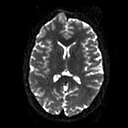
\includegraphics{eps/pepolar_vs_product/product} &
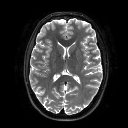
\includegraphics{eps/pepolar_vs_product/fse} &
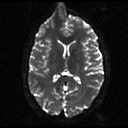
\includegraphics{eps/pepolar_vs_product/pepolar} \\
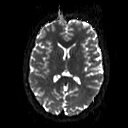
\includegraphics{eps/pepolar_vs_product/product_corrected} && 
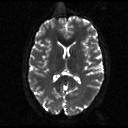
\includegraphics{eps/pepolar_vs_product/pepolar_corrected}
\end{tabular}
\end{center}
\caption{Comparison of distortion in GE product DWI acquisition vs. ``PE
  Polar'' acquisition. {\em Top row:\/} data as acquired. {\em Bottom row:\/
    data corrected for EPI distortion using either Field Map (product
    sequence, left column) or the unwarping workflow described herein (right
    column).}}
\label{fig:PEPolarVsProduct}
\end{figure}

It is readily apparent that the product DWI acquisition is less distorted to
begin with. This is due to accelerated readout in the product sequence, which
reduces the time during which signal phase is affected, thus reducing the
amount of distortion observed. Visually, the field map-corrected product
sequence image appears almost as similar to the reference FSE image as the
corrected ``PE Polar'' image.

The magnitude of this observed improvement should be weighed against the
difficulty of implementing the PE Polar acquisition technique when deciding
for or against either acquisition scheme.

\bibliographystyle{UnwarpEchoPlanar}
\bibliography{UnwarpEchoPlanar}

\end{document}

